\subsection{Task 2: supporting material}
\label{app:t2}
% Numbers: kode/results/task2/*.json (python run_all.py --task 2).

\begin{figure}[!htbp]
  \centering
  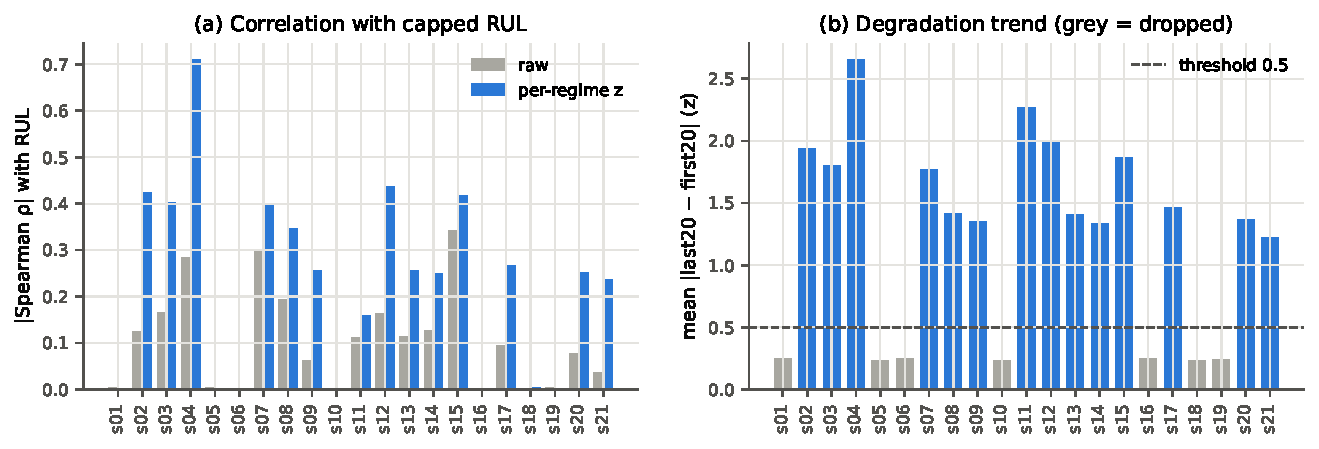
\includegraphics[width=\linewidth]{t2_sensors}
  \caption{(a) $|$Spearman $\rho|$ between each sensor and the capped RUL, before and after per-regime
  normalisation. (b) Mean absolute change between a machine's first and last 20 cycles; grey sensors are
  dropped (threshold 0.5 $z$, fitted on training machines; the same 14 sensors are kept in every fold).}
  \label{fig:t2-sensors}
\end{figure}

\begin{figure}[!htbp]
  \centering
  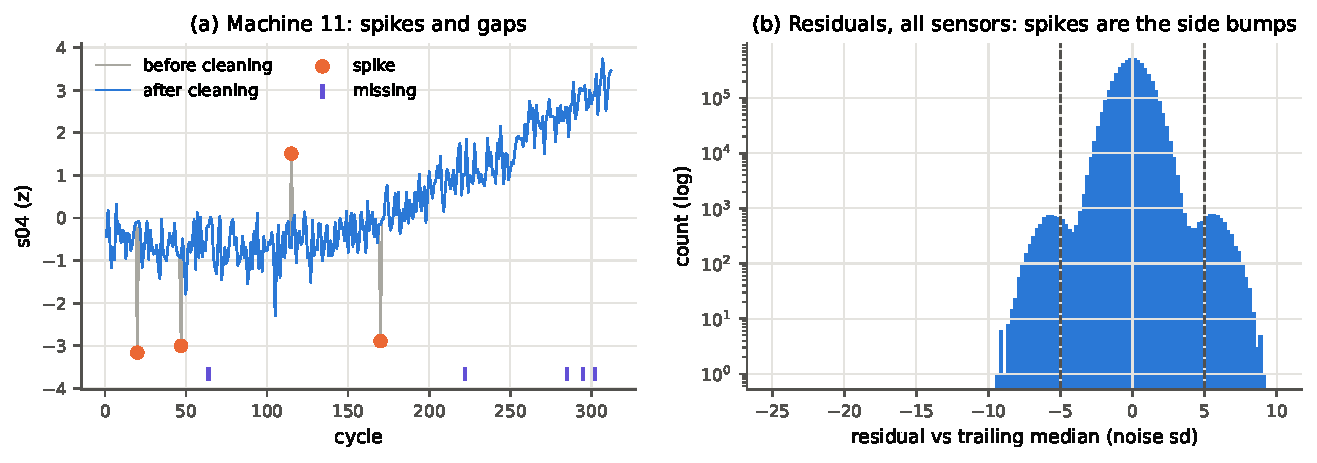
\includegraphics[width=\linewidth]{t2_missing_spikes}
  \caption{(a) One machine before and after cleaning, with detected spikes and missing readings.
  (b) Residuals from the median of the previous 10 cycles for all sensors (log scale). The side bumps are
  spikes (51\% upward, median size 3.8 $z$); the dashed lines mark the threshold of $\pm 5$ noise standard
  deviations.}
  \label{fig:t2-spikes}
\end{figure}

\begin{figure}[!htbp]
  \centering
  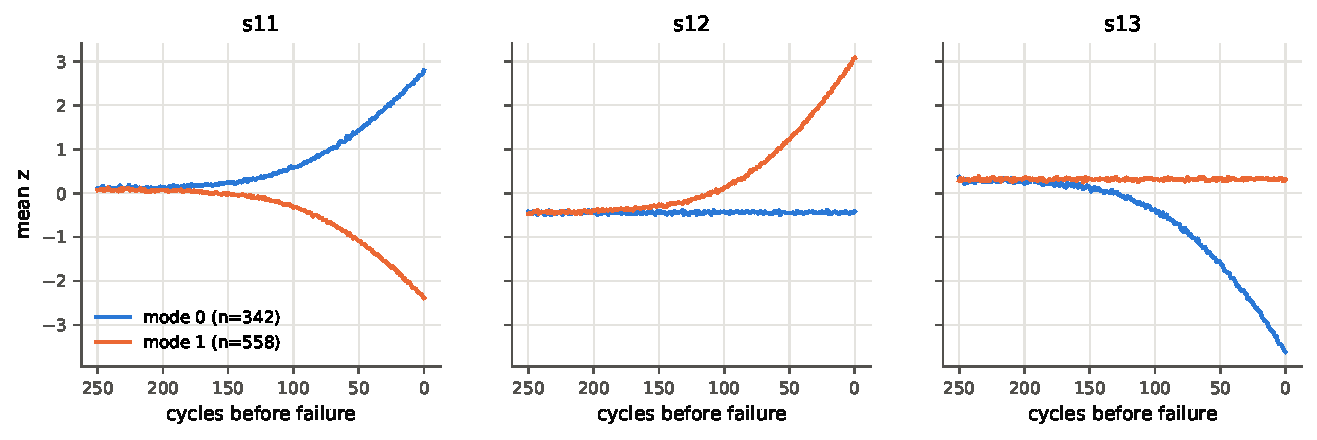
\includegraphics[width=\linewidth]{t2_failure_modes}
  \caption{Mean normalised reading against cycles before failure for the two failure modes.}
  \label{fig:t2-modes}
\end{figure}

\begin{figure}[!htbp]
  \centering
  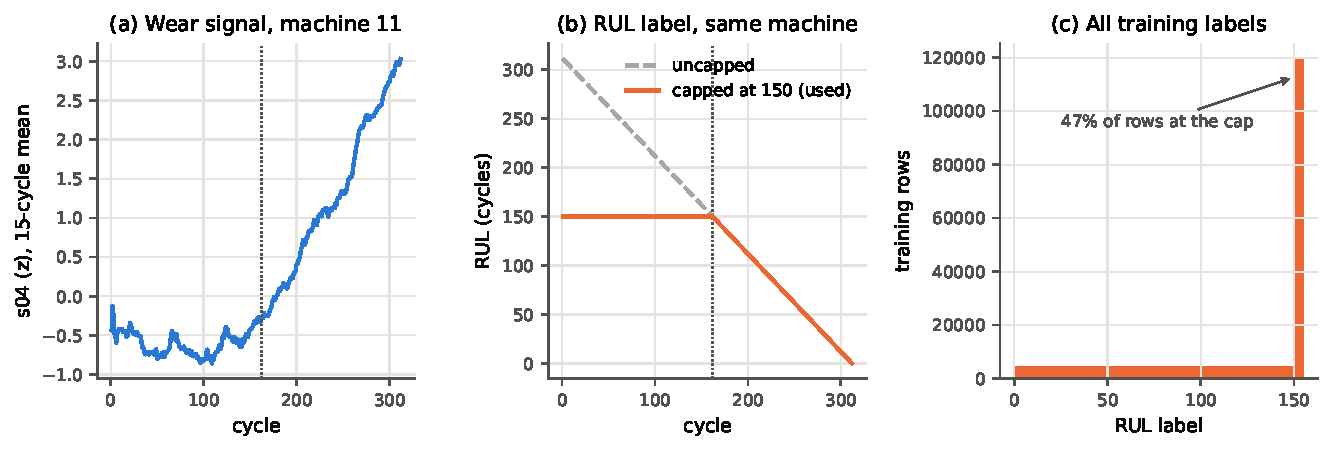
\includegraphics[width=\linewidth]{t2_labels}
  \caption{(a) Smoothed wear signal of one machine. (b) Its RUL label, uncapped and capped; the dotted line
  marks where the capped label starts to fall. (c) Distribution of all training labels.}
  \label{fig:t2-labels}
\end{figure}

\begin{figure}[!htbp]
  \centering
  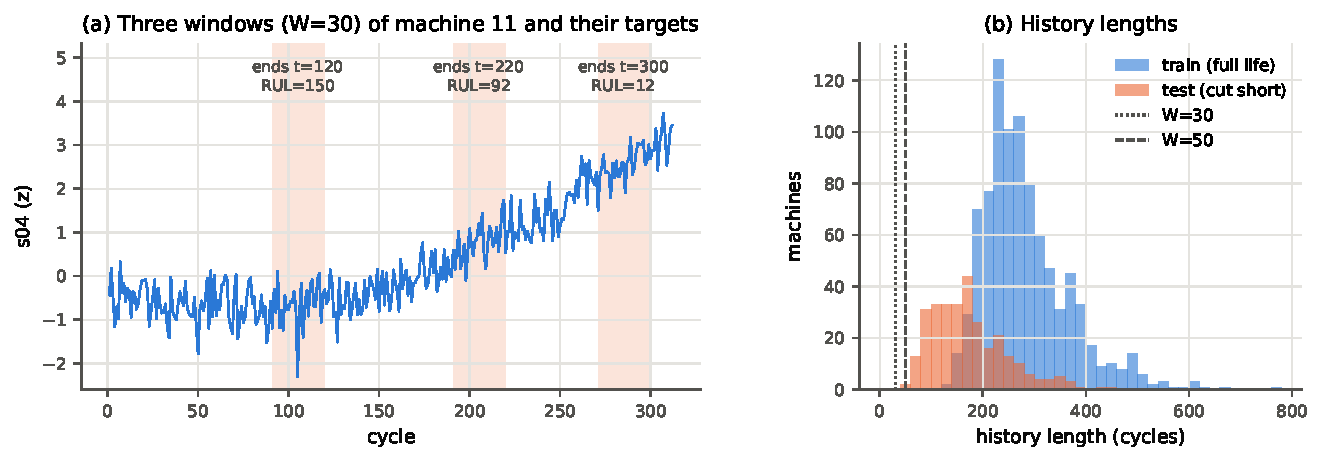
\includegraphics[width=\linewidth]{t2_windows}
  \caption{(a) Three windows of $W=30$ cycles from one machine and their targets. (b) History lengths of
  training machines (full life) and test machines (cut before failure), with the window lengths compared.}
  \label{fig:t2-windows}
\end{figure}

\begin{table}[!htbp]
  \centering
  \caption{Baselines on the 180 held-out machines ($W=30$). ``Worst 5\%'' is the share of the total
  asymmetric score caused by the worst 5\% of predictions.}
  \label{tab:t2-baseline}
  \small
  \begin{tabular}{lrrrrr}
    \toprule
    Model & RMSE & Score mean & Score median & Worst 5\% & Train RMSE \\
    \midrule
    Ridge          & 23.3 & 37.2 & 1.94 & 78\% & 20.1 \\
    Boosted trees  & 21.9 & 62.0 & 1.21 & 90\% & 14.1 \\
    \bottomrule
  \end{tabular}
\end{table}

\begin{figure}[!htbp]
  \centering
  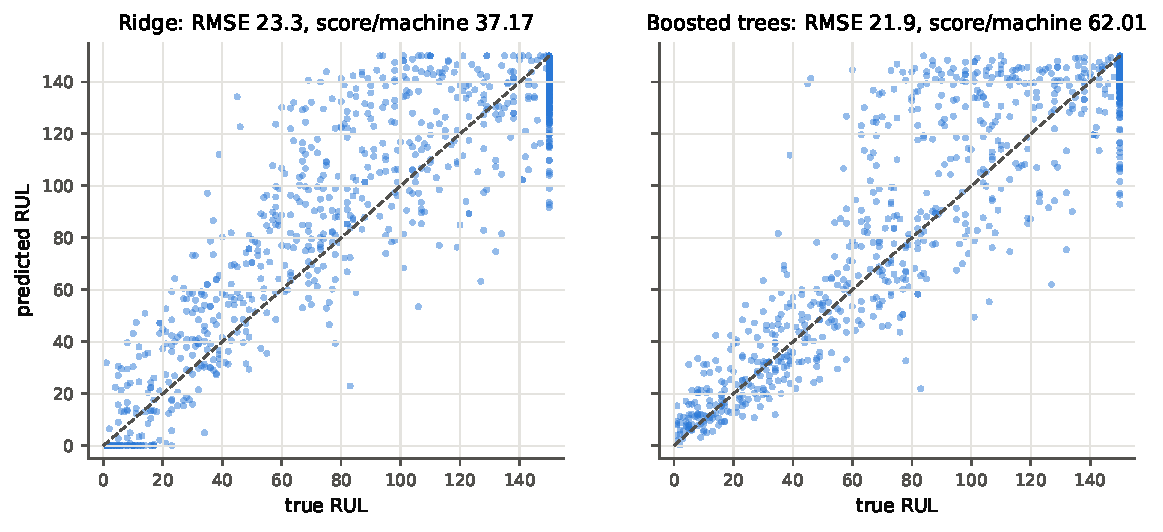
\includegraphics[width=0.85\linewidth]{t2_baseline}
  \caption{Predicted vs.\ true RUL of the baselines at the test-like cuts of the held-out machines. Points
  above the diagonal are late (over-optimistic) predictions.}
  \label{fig:t2-baseline}
\end{figure}

\begin{table}[!htbp]
  \centering
  \caption{Deep model variants, three seeds each. ``Early stop'' is the best RMSE on the 72 held-aside
  training machines (used for the choice); the other columns are on the 180 held-out machines.}
  \label{tab:t2-cnn}
  \small
  \begin{tabular}{lrrrr}
    \toprule
    Variant & Params & Early stop & RMSE & Score mean \\
    \midrule
    CNN, original ($W=30$)              & 156k & 22.35 & $22.93 \pm 0.60$ & $45 \pm 20$ \\
    CNN, pooled head                    &  37k & 24.50 & $24.11 \pm 0.82$ & $49 \pm 10$ \\
    CNN, dropout 0.5 + weight decay     & 156k & 22.43 & $22.77 \pm 0.45$ & $30 \pm 5$ \\
    CNN, longer window ($W=50$)         & 238k & 21.10 & $21.45 \pm 0.63$ & $32 \pm 8$ \\
    GRU ($W=30$)                        &  45k & 21.04 & $21.59 \pm 0.10$ & $40 \pm 1$ \\
    GRU ($W=50$)                        &  45k & 20.15 & $20.70 \pm 0.10$ & $34 \pm 6$ \\
    \bottomrule
  \end{tabular}
\end{table}

\begin{figure}[!htbp]
  \centering
  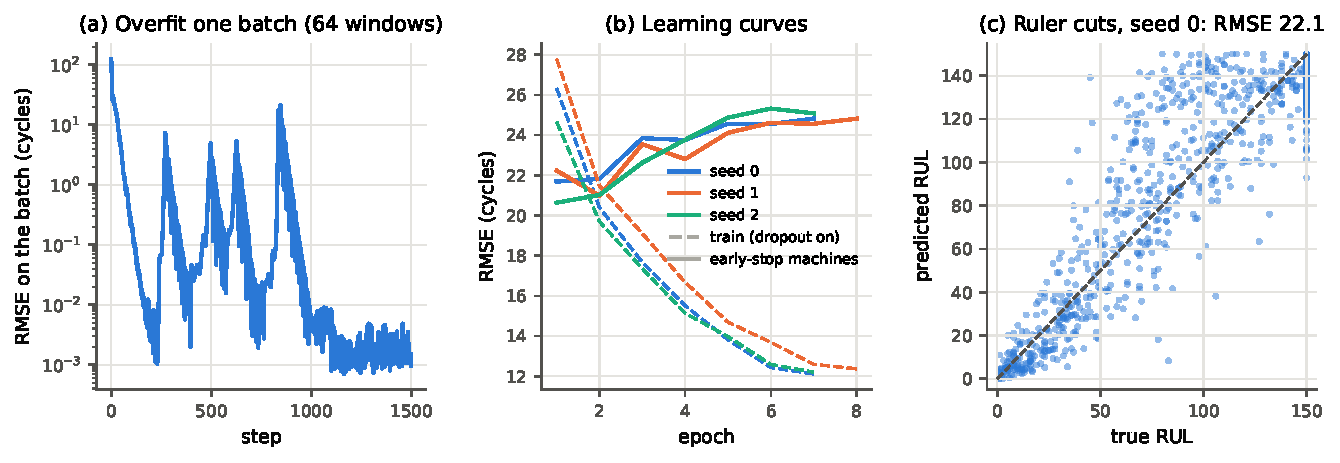
\includegraphics[width=\linewidth]{t2_cnn_W50}
  \caption{1D-CNN with $W=50$. (a) Overfitting a single batch. (b) Learning curves of three seeds (dashed:
  training, with dropout on; solid: early-stopping machines). (c) Predicted vs.\ true RUL on the held-out
  machines (seed 0).}
  \label{fig:t2-cnn}
\end{figure}

\begin{figure}[!htbp]
  \centering
  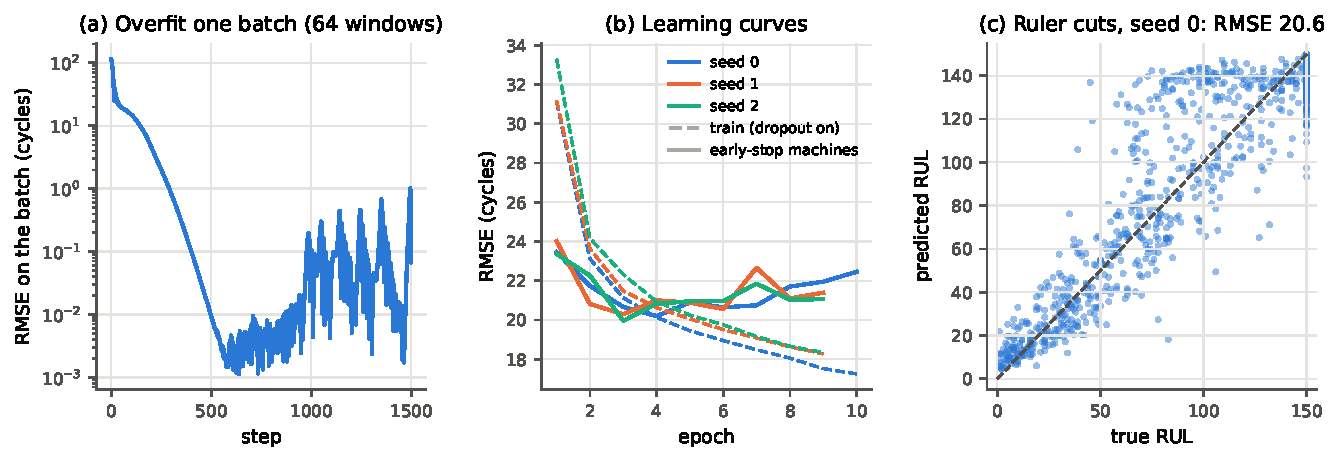
\includegraphics[width=\linewidth]{t2_gru_W50}
  \caption{GRU with $W=50$, same panels as Fig.~\ref{fig:t2-cnn}.}
  \label{fig:t2-gru}
\end{figure}

\begin{table}[!htbp]
  \centering
  \caption{90\% prediction intervals of the GRU ($W=50$) on the 180 held-out machines: coverage (share of
  true RUL inside) and mean width in cycles. Calibration uses the 72 held-aside machines, which also chose
  the best epoch but were never used to fit weights.}
  \label{tab:t2-unc}
  \small
  \begin{tabular}{lrrrr}
    \toprule
    & \multicolumn{2}{c}{Raw} & \multicolumn{2}{c}{Calibrated} \\
    Method & Coverage & Width & Coverage & Width \\
    \midrule
    MC dropout (1 net, 50 passes)         & 52\% & 22 & 89\% & 54 \\
    Ensemble (5 nets)                     & 20\% & 10 & 89\% & 61 \\
    Ensemble + MC dropout (5 $\times$ 20) & 63\% & 27 & 90\% & 50 \\
    Constant width                        & --   & -- & 89\% & 54 \\
    \bottomrule
  \end{tabular}
\end{table}

\begin{table}[!htbp]
  \centering
  \caption{Effect of lowering every prediction by a fixed shift, over 2{,}000 simulated test sets of 300
  validation machines (median change compared with no shift). Net benefit: score gain minus RMSE cost, each
  divided by its spread between test sets without shift (RMSE 1.14; summed score 4{,}658).}
  \label{tab:t2-shift}
  \small
  \begin{tabular}{rrrr}
    \toprule
    Shift (cycles) & RMSE change & Summed score change & Net benefit \\
    \midrule
    2  & $+0.02$ & $-15\%$ & $+0.20$ \\
    \textbf{3} & $\mathbf{+0.10}$ & $\mathbf{-22\%}$ & $\mathbf{+0.22}$ \\
    4  & $+0.23$ & $-27\%$ & $+0.18$ \\
    6  & $+0.63$ & $-36\%$ & $-0.04$ \\
    13 & $+3.19$ & $-50\%$ & $-2.10$ \\
    \bottomrule
  \end{tabular}
\end{table}
